\documentclass[aspectratio=169,11pt]{beamer}

\usetheme{Madrid}
\usecolortheme{default}
\usefonttheme{professionalfonts}
\setbeamertemplate{navigation symbols}{}
\setbeamertemplate{footline}[frame number]

\usepackage{amsmath, amssymb, booktabs, graphicx}
\graphicspath{{../../assets/figures/}{assets/figures/}}

\title{Synthesis, Student Research Designs, and the Bridge to Labor II}
\subtitle{Labor I -- Week 13}
\author{Teaching deck draft}
\date{}

\begin{document}

\begin{frame}
  \titlepage
\end{frame}

\begin{frame}{Why Week 13 is a synthesis and research-design week}
\begin{itemize}
    \item Labor I has built the worker side of labor economics: labor supply, human capital, job value, households, inequality, discrimination, mobility, policy, and behavioral wedges.
    \item Week 13 converts topic mastery into research capability.
    \item The capstone question is: what is the object, what is the mechanism, what design isolates it, and when do firms or equilibrium responses become central?
\end{itemize}
\end{frame}

\begin{frame}{The full Labor I architecture}
\begin{itemize}
    \item Week 1: measurement and labor-market objects.
    \item Weeks 2--3: static and dynamic worker choice.
    \item Weeks 4--5: skill accumulation, wages, and returns.
    \item Weeks 6--7: households, care, amenities, and total job value.
    \item Weeks 8--10: inequality, discrimination, sorting, and mobility.
    \item Weeks 11--12: policy design, behavioral wedges, and interpretation.
\end{itemize}
\end{frame}

\begin{frame}{Unified worker-side framework}
\[
V_{it}(x_{it})
=
\max_{h_t,s_t,j_t,m_t}
\left\{
u(c_t,1-h_t,a_{j_t},\ell_t;\theta_i)
- \chi_i(h_t,s_t,m_t)
+ \beta \mathbb{E}_t[V_{i,t+1}(x_{i,t+1})]
\right\}
\]

\[
k_{i,t+1} = g(k_{it}, s_t, x_{it}, \varepsilon_{i,t+1})
\qquad
J_{ij} = w_{ij} + A_{ij} - C_{ij}
\]

\begin{itemize}
    \item Hours, skill investment, job choice, and mobility are the recurring Labor I margins.
    \item Policy, household structure, information, and behavioral wedges shift the feasible set or the perceived set.
\end{itemize}
\end{frame}

\begin{frame}{Human capital is the dynamic backbone}
\begin{center}
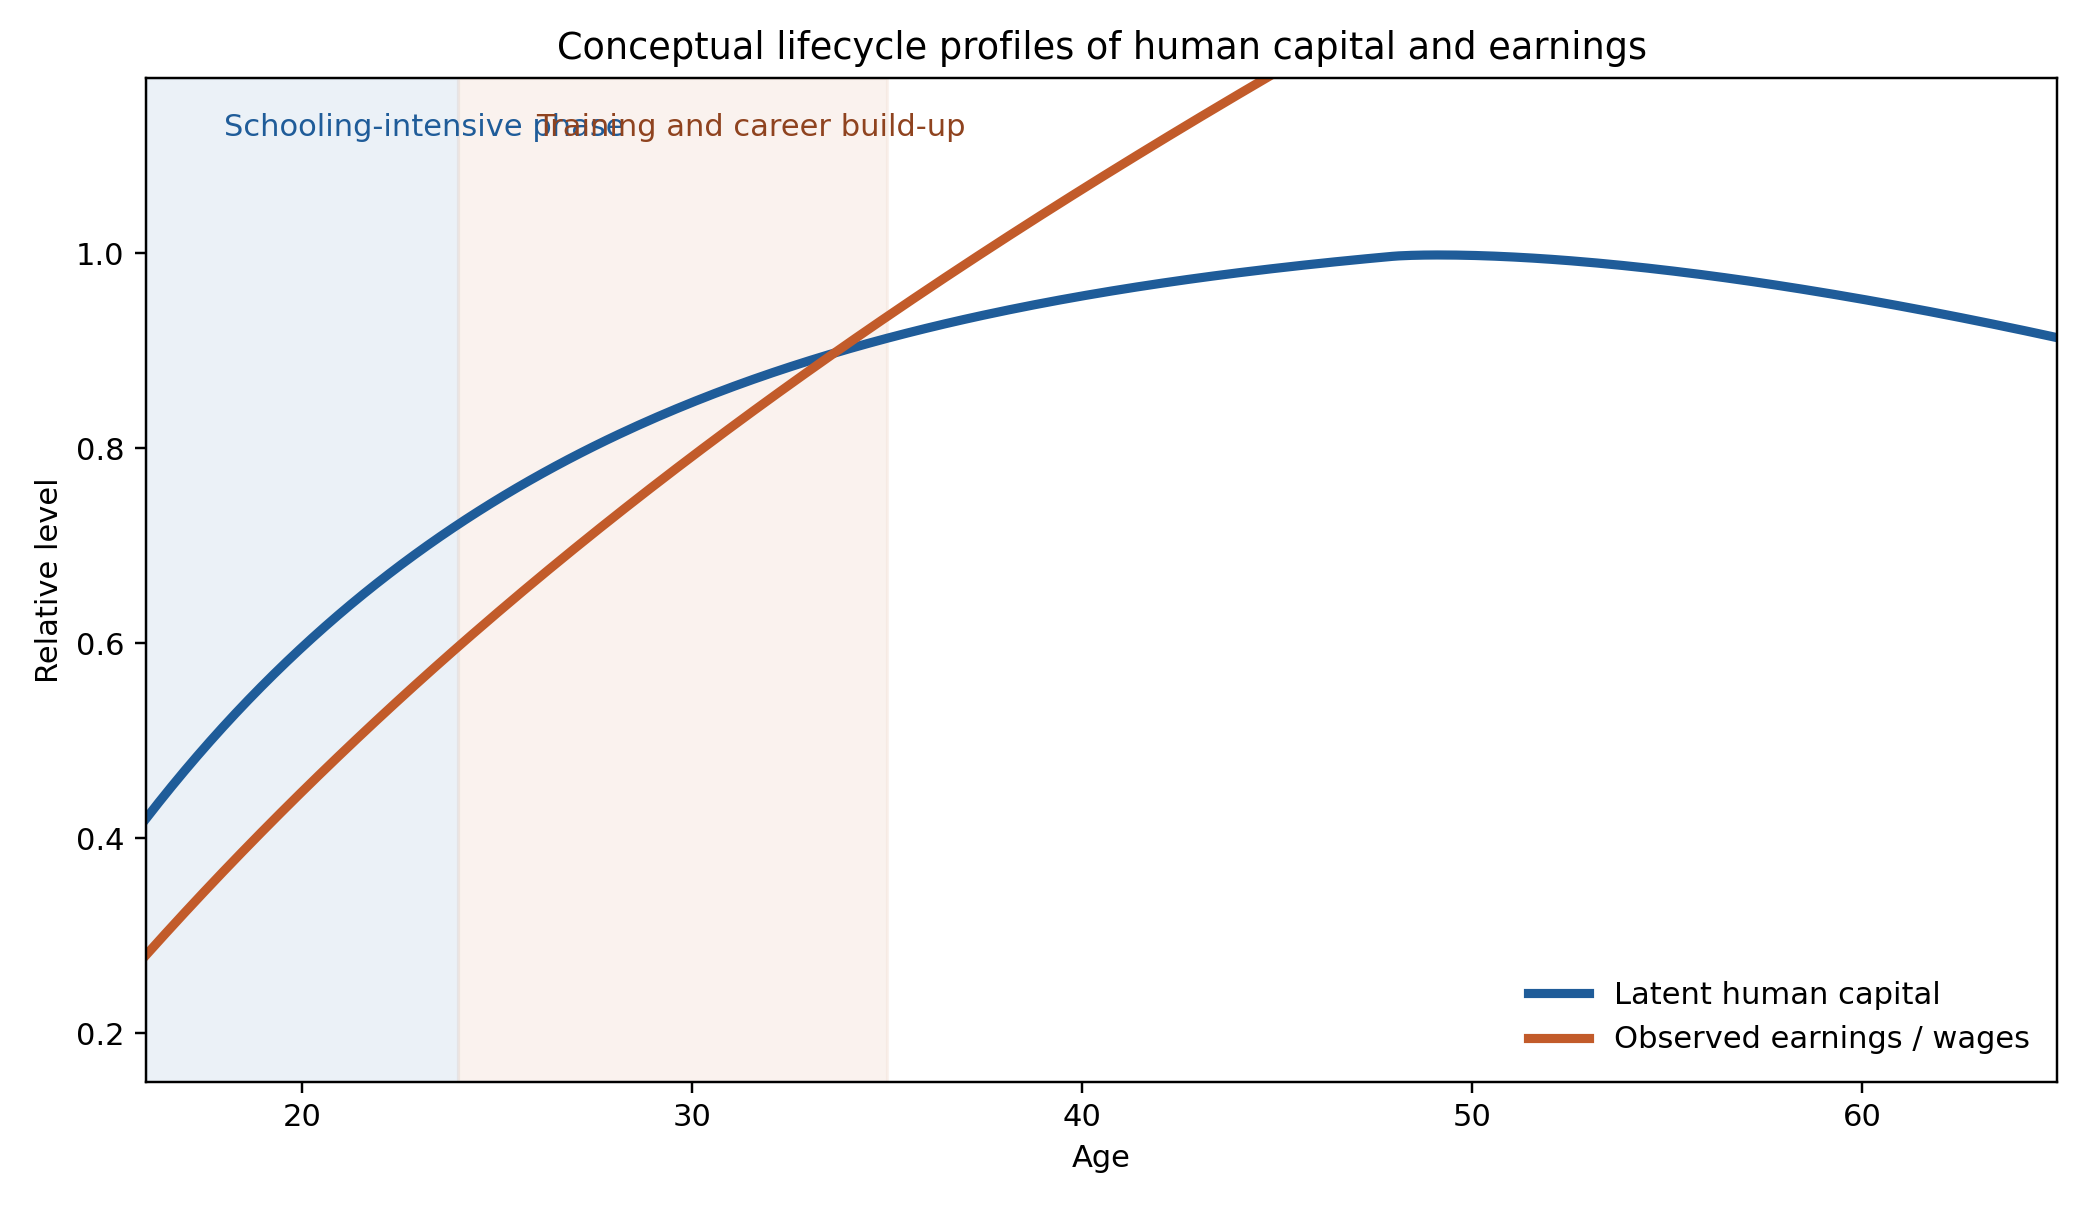
\includegraphics[height=0.72\textheight,keepaspectratio]{04-lifecycle-human-capital-earnings.png}
\end{center}
\end{frame}

\begin{frame}{Wages are not the whole object}
\begin{center}
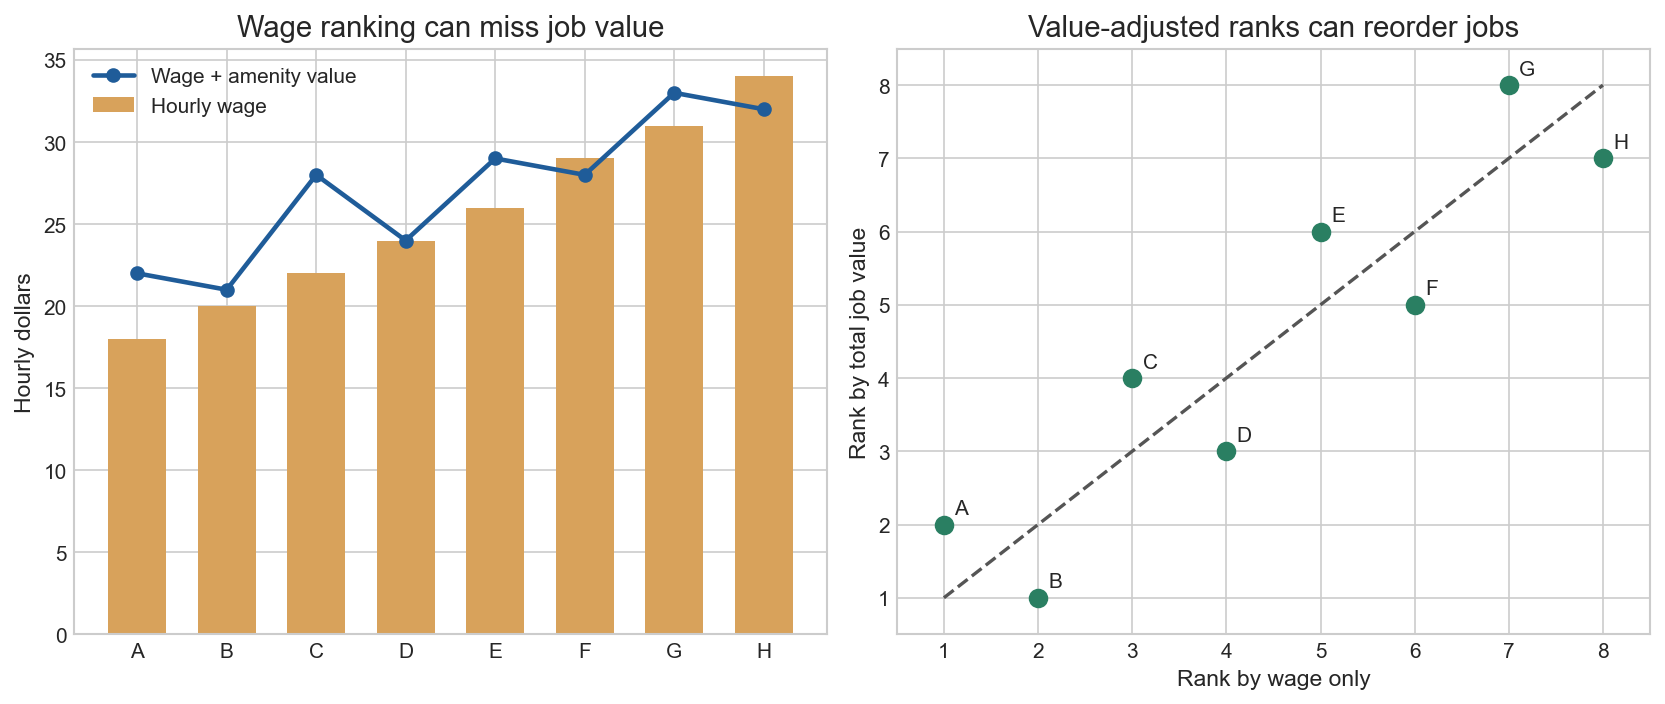
\includegraphics[height=0.72\textheight,keepaspectratio]{07-wage-inequality-total-job-value.png}
\end{center}
\end{frame}

\begin{frame}{What makes a good labor research question?}
\begin{itemize}
    \item A topic is not a question.
    \item A descriptive pattern is not a mechanism.
    \item A mechanism is not an identification strategy.
    \item A good labor question names one object, one mechanism, one population, and one contribution.
    \item A good Week 13 question also says whether it is partial equilibrium or already needs Labor II tools.
\end{itemize}
\end{frame}

\begin{frame}{Mechanism--data--design--contribution pipeline}
\[
\tau = \mathbb{E}[Y_i(1)-Y_i(0)]
\qquad
P(j \mid i) = f(k_i,z_i,a_j,w_j,d_{ij})
\]

\begin{itemize}
    \item Object: what outcome or estimand do we care about?
    \item Mechanism: what margin is supposed to move?
    \item Data: which unit and which measurement technology fit the object?
    \item Design: what variation or model discipline isolates the mechanism?
    \item Contribution: what would labor economists understand differently if the result were true?
\end{itemize}
\end{frame}

\begin{frame}{The design problem is a matching problem}
\begin{center}
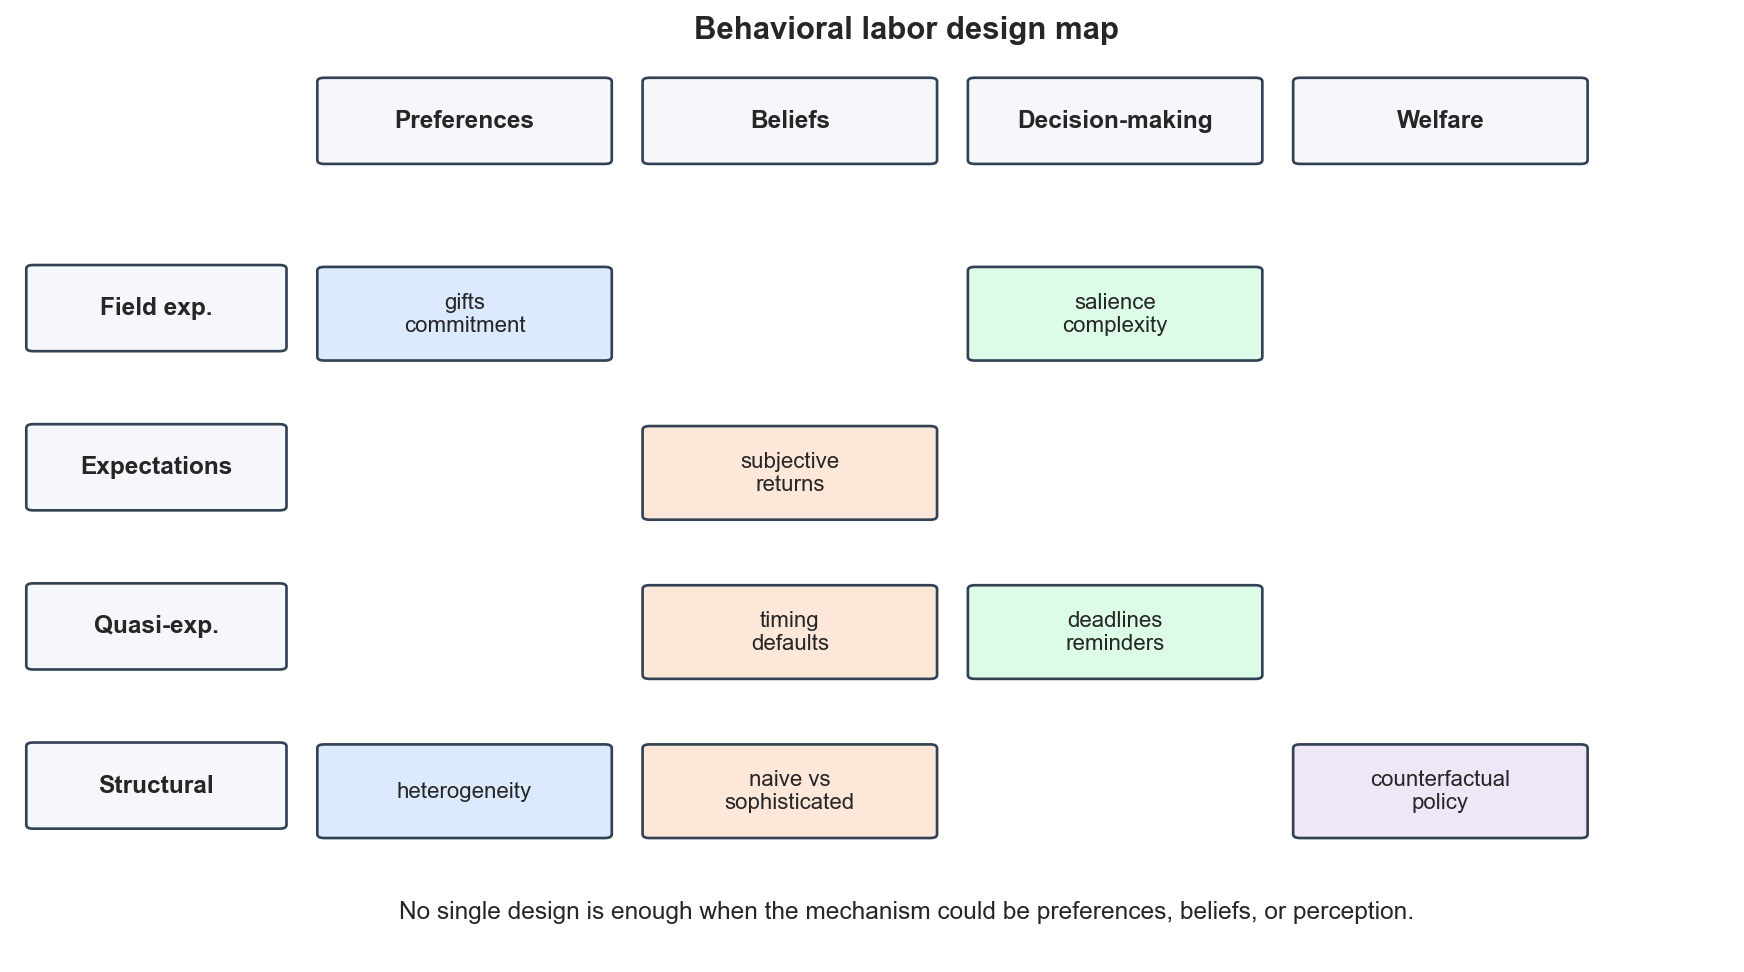
\includegraphics[height=0.72\textheight,keepaspectratio]{12-behavioral-labor-design-map.png}
\end{center}
\end{frame}

\begin{frame}{Example research templates}
\begin{itemize}
    \item Labor supply under schedule volatility, benefit design, or information.
    \item Human-capital investment under beliefs, liquidity, or timing frictions.
    \item Wage determination with selection, sorting, or firm premia.
    \item Household and care responses to policy or shocks.
    \item Job amenities, flexibility, and total job value.
    \item Inequality, discrimination, mobility, and behavioral response.
\end{itemize}
\end{frame}

\begin{frame}{Common Week 13 failure modes}
\begin{itemize}
    \item Topic without a question.
    \item Mechanism without design.
    \item Design without labor contribution.
    \item Too many outcomes and no primary estimand.
    \item Hidden equilibrium issue.
    \item Literature survey posing as an idea.
\end{itemize}
\end{frame}

\begin{frame}{Inequality is an accumulation and assignment outcome}
\begin{center}
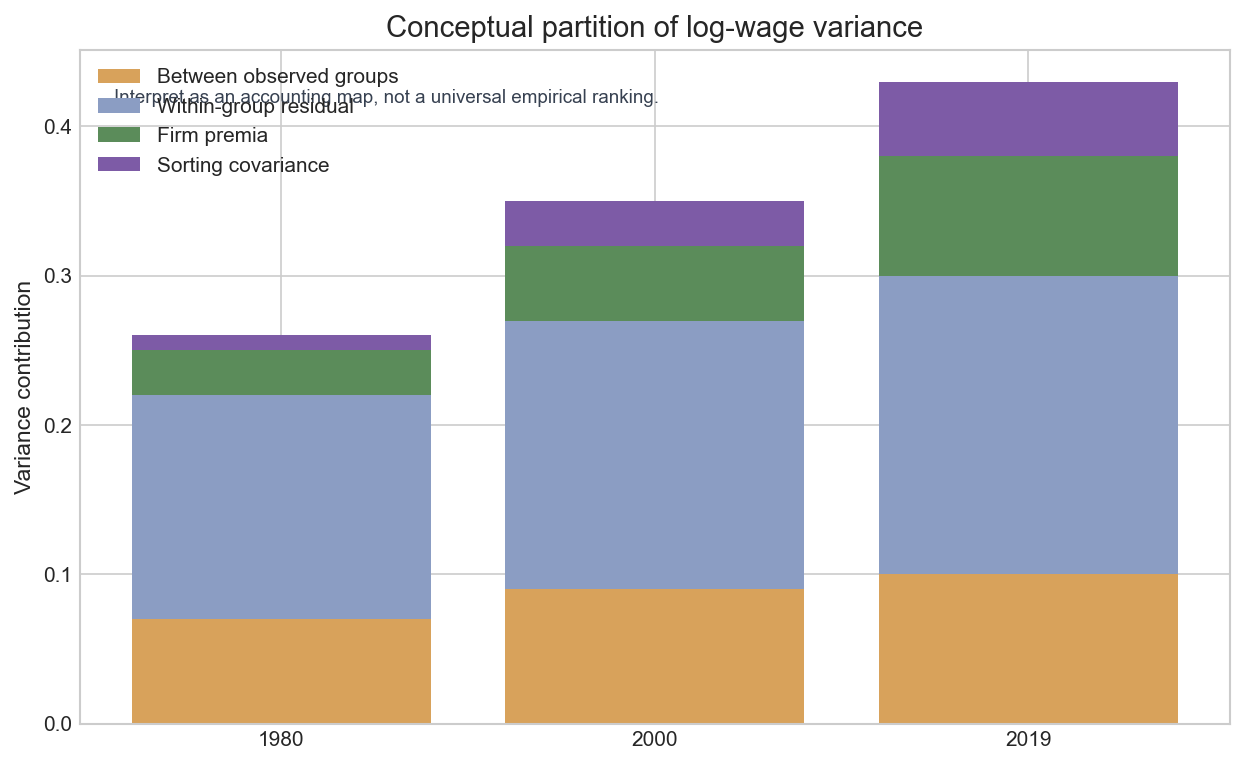
\includegraphics[height=0.72\textheight,keepaspectratio]{08-inequality-component-decomposition.png}
\end{center}
\end{frame}

\begin{frame}{Bridge to Labor II}
\[
w_{ij} = \phi_i + \psi_j + \varepsilon_{ij}
\qquad \text{or} \qquad
M(U,V)
\]

\begin{itemize}
    \item Labor I asks how workers choose, invest, sort, and respond.
    \item Labor II asks what changes once firms choose wages, vacancies, schedules, training, and organizational rules.
    \item Search frictions, monopsony, personnel economics, institutions, and aggregate adjustment all live on this bridge.
\end{itemize}
\end{frame}

\begin{frame}{Where Labor I becomes Labor II}
\begin{center}
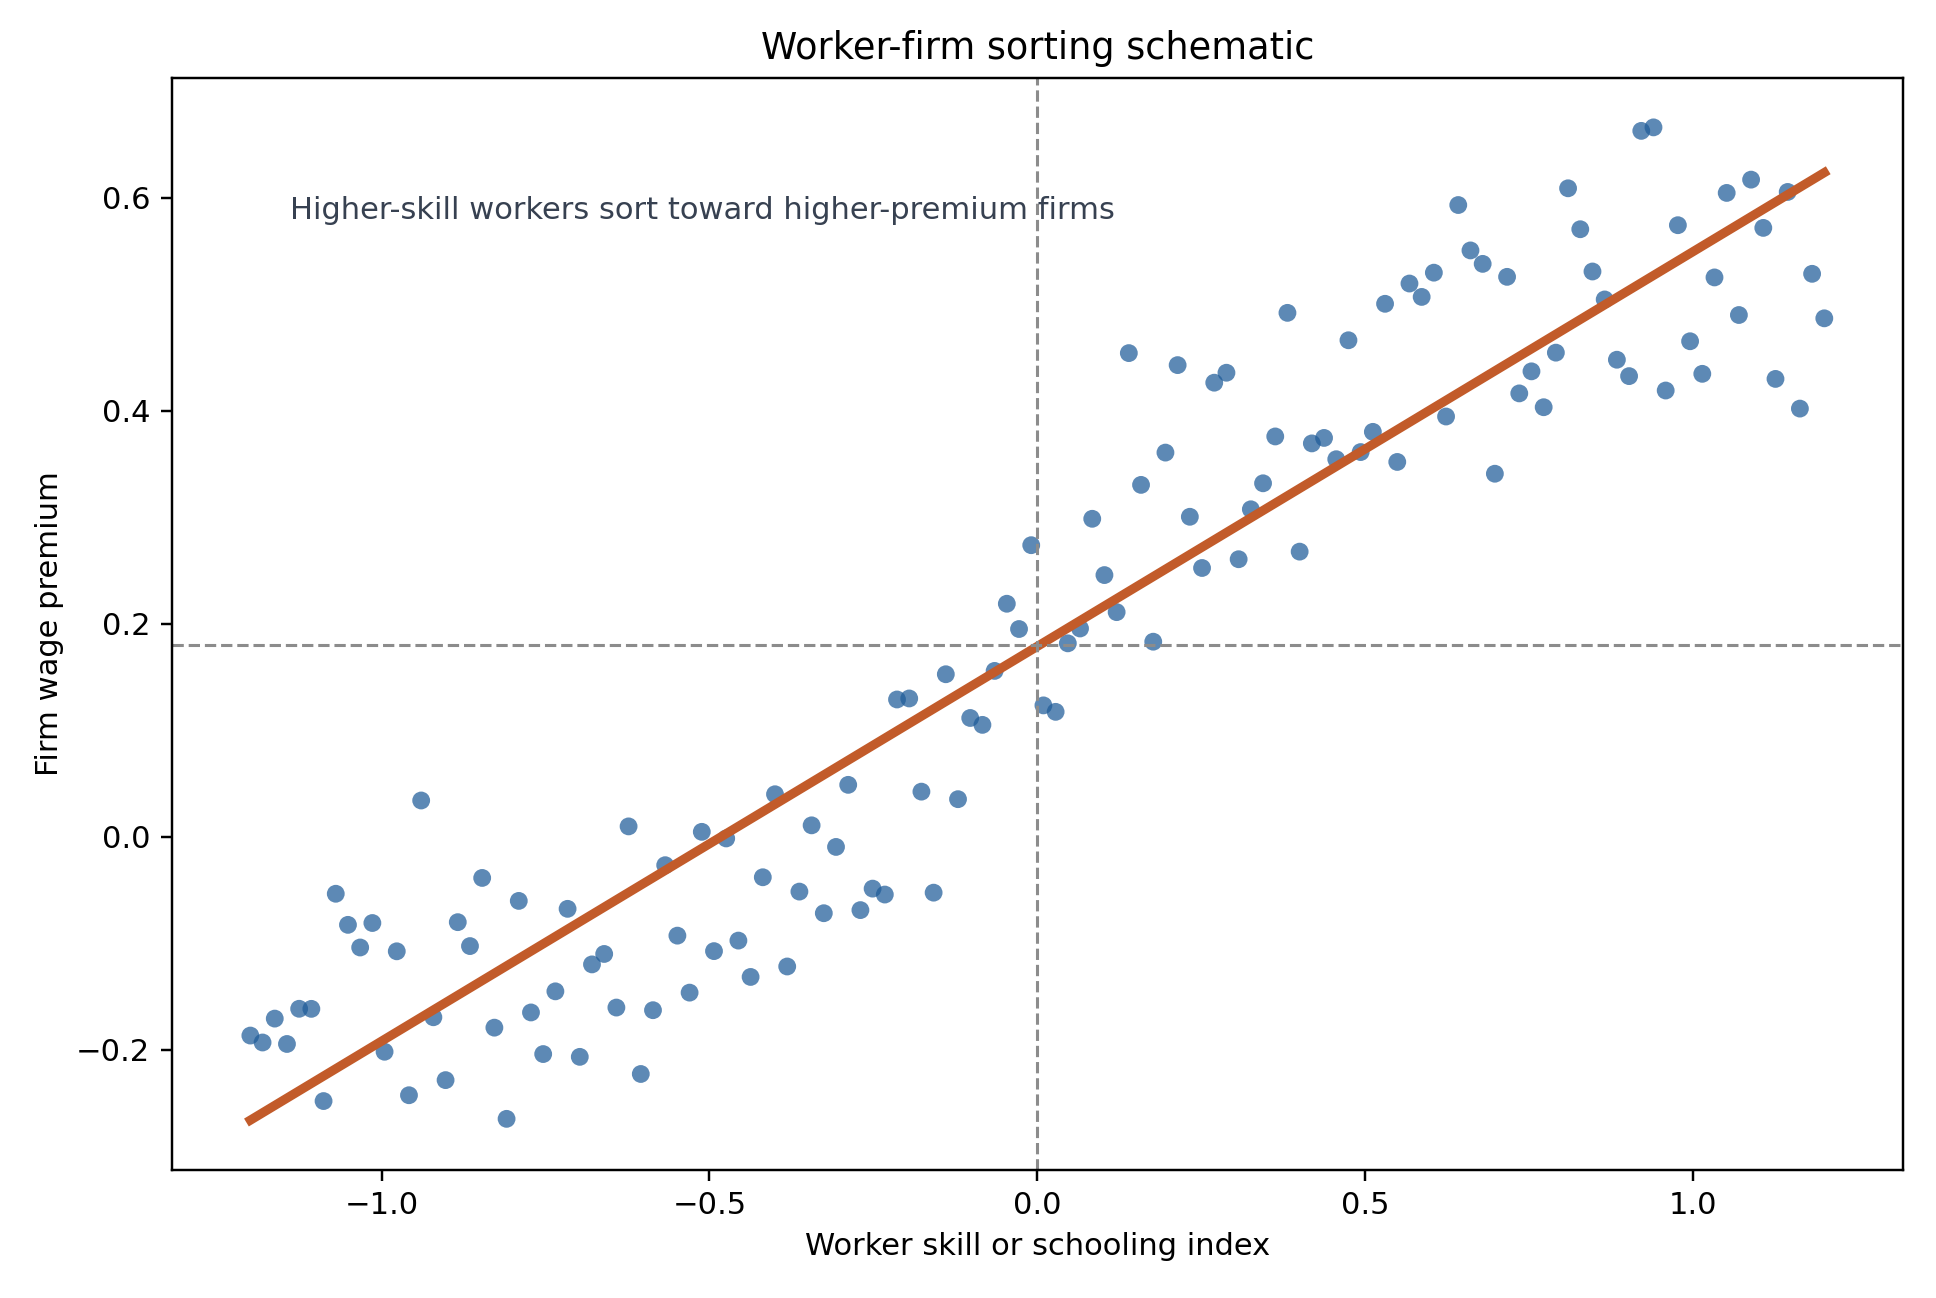
\includegraphics[height=0.72\textheight,keepaspectratio]{05-worker-firm-sorting-schematic.png}
\end{center}
\end{frame}

\begin{frame}{Student memo template}
\begin{itemize}
    \item One sentence: ``This paper asks...''
    \item One paragraph on the object and the population.
    \item One paragraph on the mechanism and the main alternative.
    \item One paragraph on data and measurement.
    \item One paragraph on design or model discipline.
    \item One paragraph on the labor contribution.
    \item One paragraph on whether the idea remains Labor I or already requires Labor II.
\end{itemize}
\end{frame}

\begin{frame}{Where Labor I fits inside modern labor economics}
\begin{itemize}
    \item Labor I is the worker-side core of the field.
    \item Modern labor economics studies worker choices jointly with firms, institutions, and shocks.
    \item The same worker-side question can become a firm-side, search, bargaining, or equilibrium question once adjustment margins are opened.
    \item Week 13 should leave students with closure on the first semester and a map for where the second semester begins.
\end{itemize}
\end{frame}

\begin{frame}{Takeaways}
\begin{itemize}
    \item Labor I is coherent once we organize it around worker-side objects and margins.
    \item Strong labor ideas move from topic to mechanism, data, design, and contribution.
    \item Many strong Labor I projects are partial-equilibrium by design, but they should name where Labor II begins.
    \item The capstone deliverable is a feasible research memo, not a giant agenda.
\end{itemize}
\end{frame}

\appendix

\begin{frame}{Appendix: anchor-paper menu}
\begin{itemize}
    \item Card (1999): returns and identification.
    \item Autor, Katz, and Kearney (2008): inequality architecture.
    \item Card et al. (2018) and Song et al. (2019): worker--firm bridge.
    \item Neumark (2018): discrimination and design discipline.
    \item DellaVigna (2009, 2018): behavioral wedge and research design.
\end{itemize}
\end{frame}

\end{document}
